\subsection{Des entrées aléatoires à une distribution}
Un générateur $g_w$ transforme une entrée aléatoire $Y\in\RR^r$ en une image $X=g_w(Y)\in\RR^d$. La loi d'entrée $\eta$, par exemple une gaussienne standard, est choisie à l'avance. La loi de sortie est la mesure image $\mu_w=(g_w)_\#\eta$. Cette notation décrit la redistribution de la masse de probabilité par le réseau. Un générateur est une transformation apprise, qui n'est généralement pas l'inverse d'un classifieur.

\begin{figure}[htbp]\centering
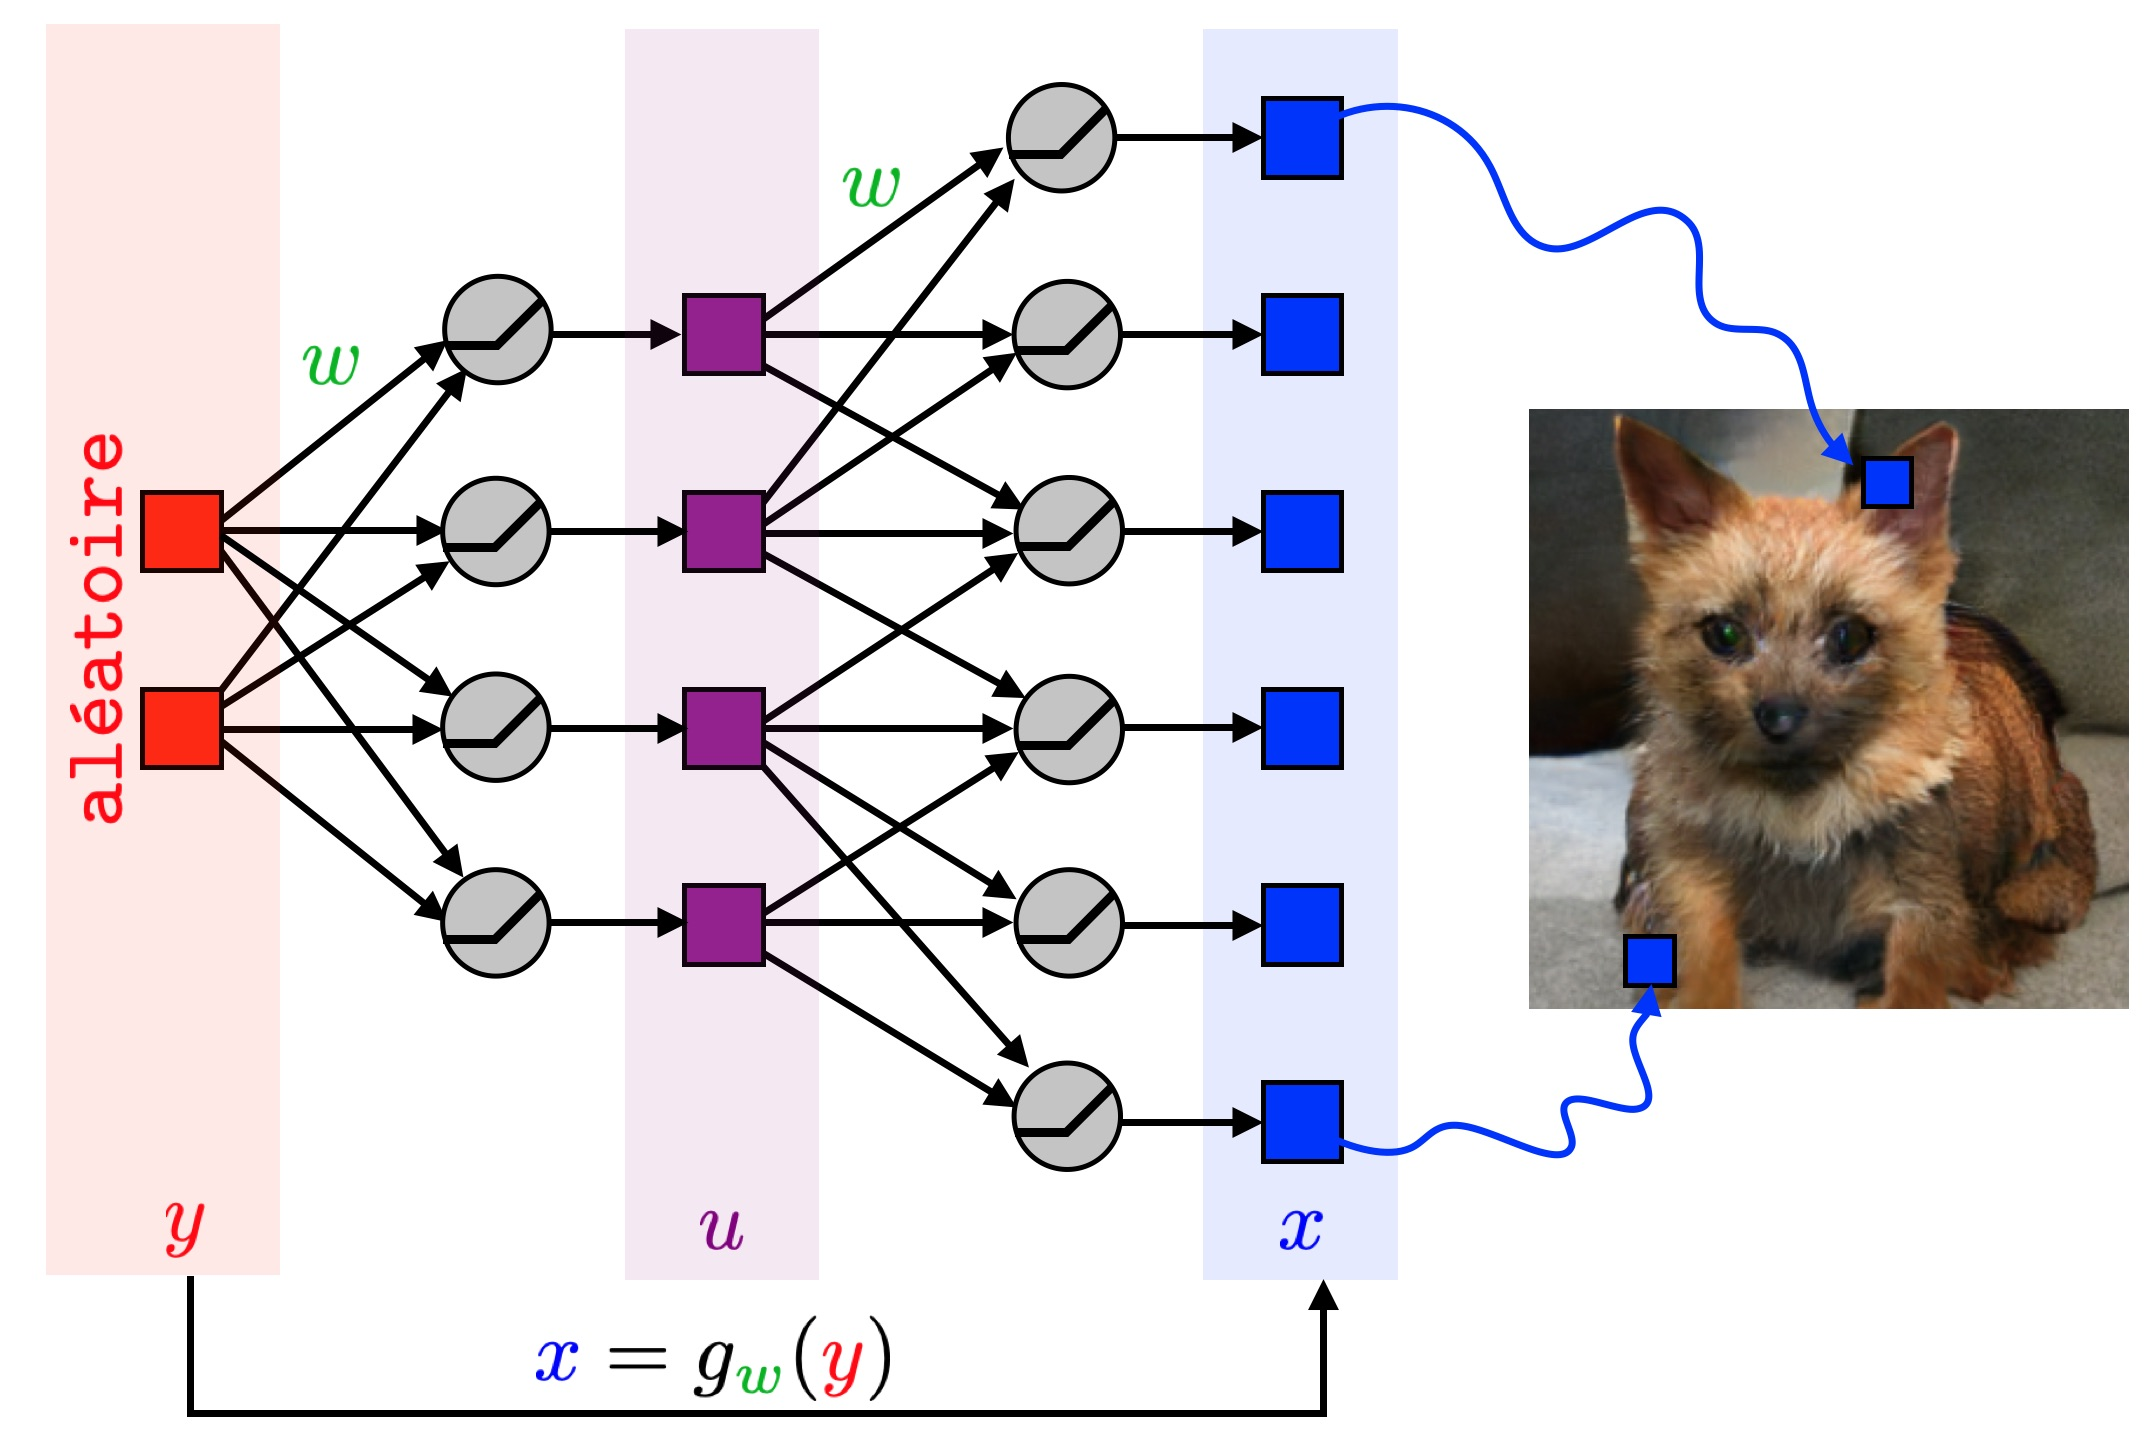
\includegraphics[width=.82\linewidth]{generative.jpg}
\caption{Un générateur schématique transforme une entrée aléatoire $y$, en passant par une couche cachée, en une image $x=g_w(y)$. Les générateurs d'images utilisés en pratique ont davantage de couches et une dimension de sortie bien plus grande.}\label{fig:generative}
\end{figure}

Pour la génération non conditionnelle, l'apprentissage peut utiliser des images sans étiquette de classe. Leur collecte, leur sélection et leur prétraitement demandent toujours de l'attention. La génération conditionnelle fournit en outre une information telle qu'une étiquette de classe, donnant un modèle $g_w(y,c)$. Tous les modèles génératifs ne sont donc pas entraînés sans supervision.

Le but est de reproduire une distribution, y compris sa diversité. Si la distribution de référence attribue une probabilité $1/2$ aux chats et $1/2$ aux chiens, un générateur idéal possède aussi ces probabilités. Un lot aléatoire fini ne contient pas nécessairement exactement la moitié de chaque catégorie. Un modèle produisant toujours la même image plausible n'a pas appris toute la distribution ; c'est une forme extrême d'effondrement des modes.

\subsection{Comparer des distributions empiriques}
\label{sec-app-gen}
Notons $z_1,\ldots,z_n$ les images d'apprentissage et $x_i=g_w(y_i)$ les images générées à partir d'échantillons latents indépendants. Leurs distributions empiriques sont
\[
 \mu_{w,n}=\frac1n\sum_{i=1}^n\delta_{x_i},\qquad
 \nu_n=\frac1n\sum_{j=1}^n\delta_{z_j}.
\]
L'emploi de mesures conserve les fréquences et les répétitions d'échantillons, que la notation ensembliste ordinaire effacerait. Un objectif possible est une distance de transport entre ces mesures.

Pour un coût euclidien, la distance de Wasserstein empirique d'ordre un vaut
\begin{equation}\label{eq-nn-w1}
 W_1(\mu_{w,n},\nu_n)
 =\frac1n\min_{s\in\Sigma_n}\sum_{i=1}^n\norm{g_w(y_i)-z_{s(i)}}_2.
\end{equation}
Le facteur $1/n$ normalise la masse totale de probabilité. Cette distance diffère du coût quadratique introduit au chapitre sur le transport. Pour des nombres d'échantillons ou des poids différents, on remplace la permutation par un couplage aux marginales prescrites.

\begin{figure}[htbp]\centering
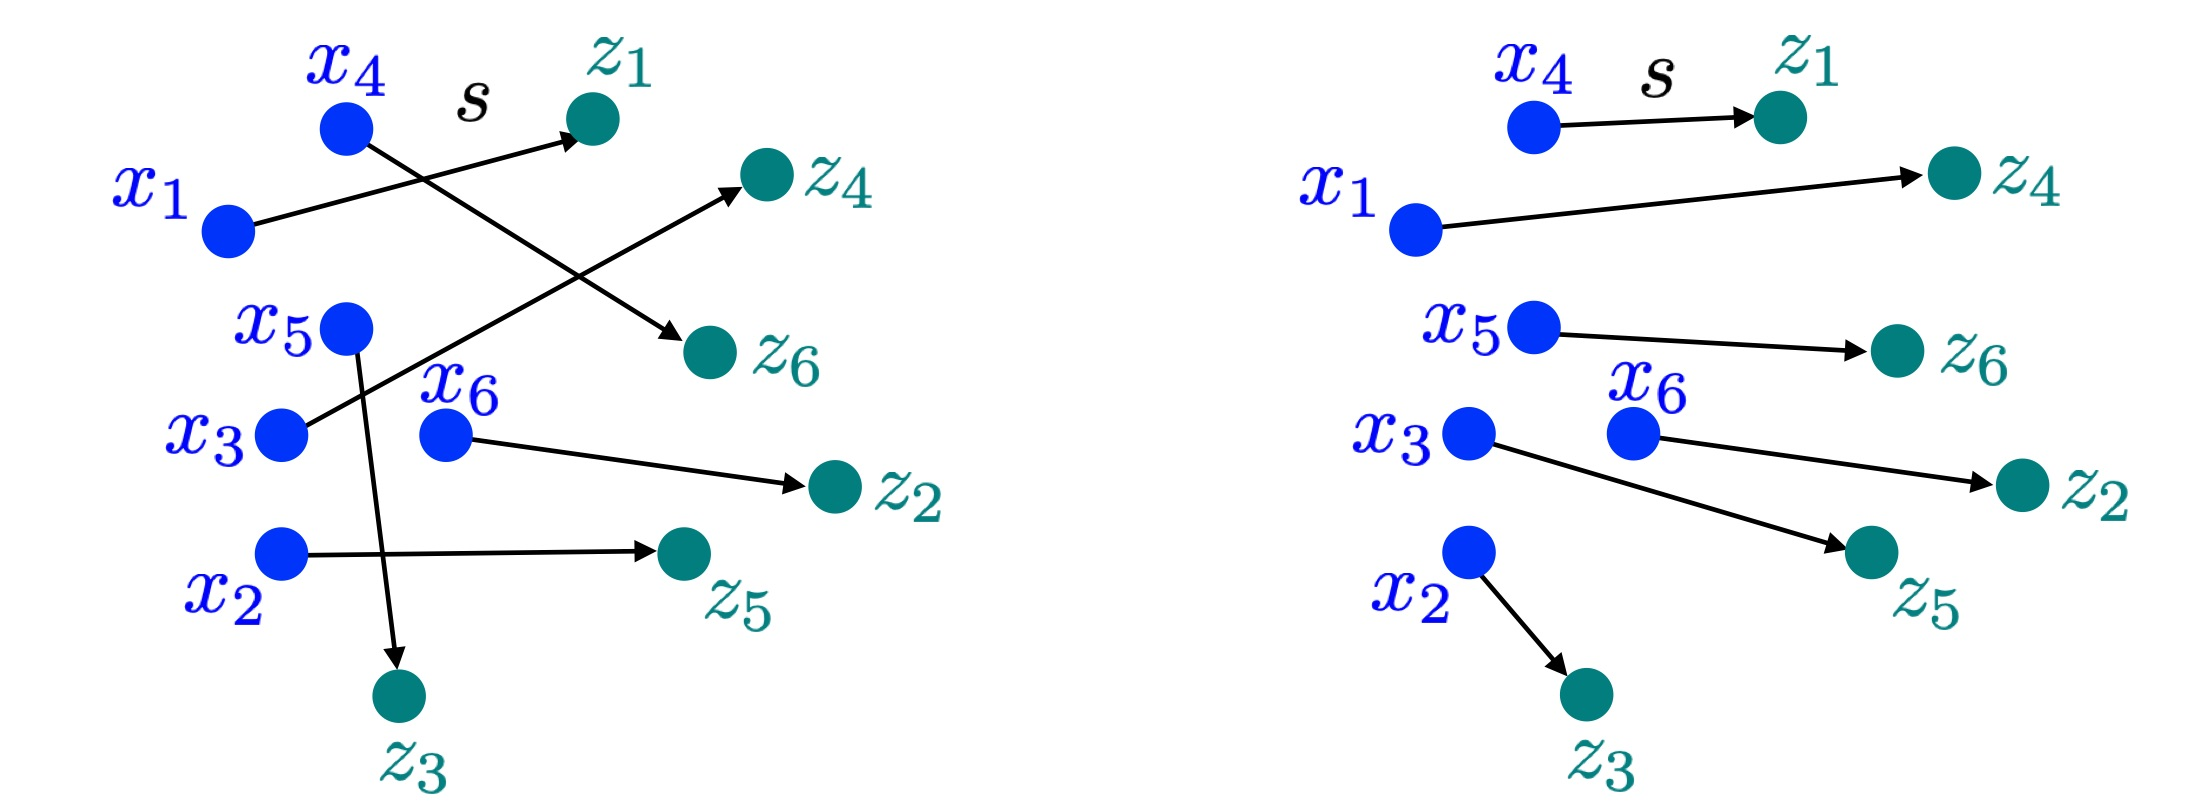
\includegraphics[width=.84\linewidth]{otmonge.jpg}
\caption{Deux affectations de six points sources à six points cibles. L'affectation de droite a un coût de transport euclidien plus faible et constitue l'appariement optimal de cet exemple.}\label{fig:otmonge}
\end{figure}

À la figure~\ref{fig:otmonge}, l'affectation de gauche est $(1,5,4,6,3,2)$, tandis que celle de droite est $(4,3,5,1,6,2)$. La notation donne la liste $(s(1),\ldots,s(6))$. Bien qu'il y ait $6!=720$ possibilités, des algorithmes d'affectation efficaces évitent l'énumération des $n!$ permutations et résolvent un problème dense en $O(n^3)$ opérations. Le chapitre sur le transport explique la relaxation convexe sous-jacente~\cite{PeyreCuturi}.

L'objectif d'apprentissage distributionnel est $\min_w W_1(\mu_w,\nu)$ pour une loi cible $\nu$. Le transport entre échantillons finis en fournit une approximation numérique, mais soulève des difficultés statistiques et d'optimisation. Le transport entre petits lots est généralement un estimateur biaisé de la distance entre les lois. L'affectation optimale peut changer avec $w$, de sorte que l'objectif empirique n'est pas partout différentiable.

La distance de base joue aussi un rôle essentiel. La distance euclidienne entre tableaux de pixels est sensible aux petites translations et peut mal refléter la similarité sémantique. Une représentation par caractéristiques peut fournir un coût plus pertinent, mais son choix modifie la géométrie apprise.

\subsection{Réseaux génératifs antagonistes}
Les réseaux génératifs antagonistes, ou GAN, introduits par Goodfellow et ses collaborateurs en 2014~\cite{goodfellow2014generative}, entraînent un générateur face à un discriminateur. Le discriminateur $D_v(x)\in(0,1)$ cherche à distinguer les données des échantillons générés. L'objectif minimax original est
\begin{equation}\label{eq-gan}
 \min_w\max_v\left\{
 \mathbb E_{Z\sim\nu}[\log D_v(Z)]
 +\mathbb E_{Y\sim\eta}[\log(1-D_v(g_w(Y)))]\right\}.
\end{equation}
Le discriminateur augmente l'objectif ; le générateur le diminue. Des mises à jour de gradient alternées approchent ce jeu, sans garantie générale de convergence pour des réseaux arbitraires.

Pour un discriminateur sans restriction et optimisé exactement, le supremum intérieur vaut $-\log4+2\operatorname{JS}(\nu,\mu_w)$, où la divergence de Jensen--Shannon est
\[
 \operatorname{JS}(\nu,\mu)=\tfrac12\operatorname{KL}(\nu\mid m)
 +\tfrac12\operatorname{KL}(\mu\mid m),\qquad m=\tfrac12(\nu+\mu).
\]
Ici, KL utilise les logarithmes naturels et se définit entre mesures à l'aide de leurs densités de Radon--Nikodym. Les deux mesures sont absolument continues par rapport à $m$. L'identité concerne l'optimum idéal du discriminateur ; des réseaux finis et une optimisation incomplète modifient l'objectif effectivement atteint. En pratique, on utilise souvent pour le générateur la perte $-\mathbb E\log D_v(g_w(Y))$, qui vise la même distribution optimale mais donne des gradients différents.

\subsection{Le lien avec Wasserstein}
Les GAN de Wasserstein~\cite{martin2017wasserstein} emploient un autre objectif, fondé sur la formule duale de Kantorovitch--Rubinstein. Pour des mesures de probabilité sur $\RR^d$ à moments d'ordre un finis,
\begin{equation}\label{eq-wgan-dual}
 W_1(\nu,\mu_w)=\sup_{\operatorname{Lip}(h)\le1}
 \left\{\mathbb E_{Z\sim\nu}h(Z)-\mathbb E_{Y\sim\eta}h(g_w(Y))\right\}.
\end{equation}
La contrainte signifie $|h(x)-h(x')|\le\norm{x-x'}_2$ pour tous $x,x'$. Un réseau critique approche cette classe de fonctions ; ses valeurs sont des scores réels, et non des probabilités de classes. Le générateur minimise l'écart estimé par le critique.

Le critique est un potentiel dual pour une distance de base \emph{fixée} ; il n'apprend pas automatiquement un nouveau coût de transport entre paires d'images. Imposer ou approcher la contrainte lipschitzienne est essentiel. La restriction de la classe des critiques et leur optimisation approchée signifient aussi que le score calculé n'est pas nécessairement égal à la véritable distance de Wasserstein.

Les GAN ordinaires et les GAN de Wasserstein expriment ainsi des principes antagonistes proches, avec des objectifs mathématiques différents. Aucune des deux procédures ne garantit que toute image générée soit pertinente ou que tous les modes soient représentés.

\begin{figure}[htbp]\centering
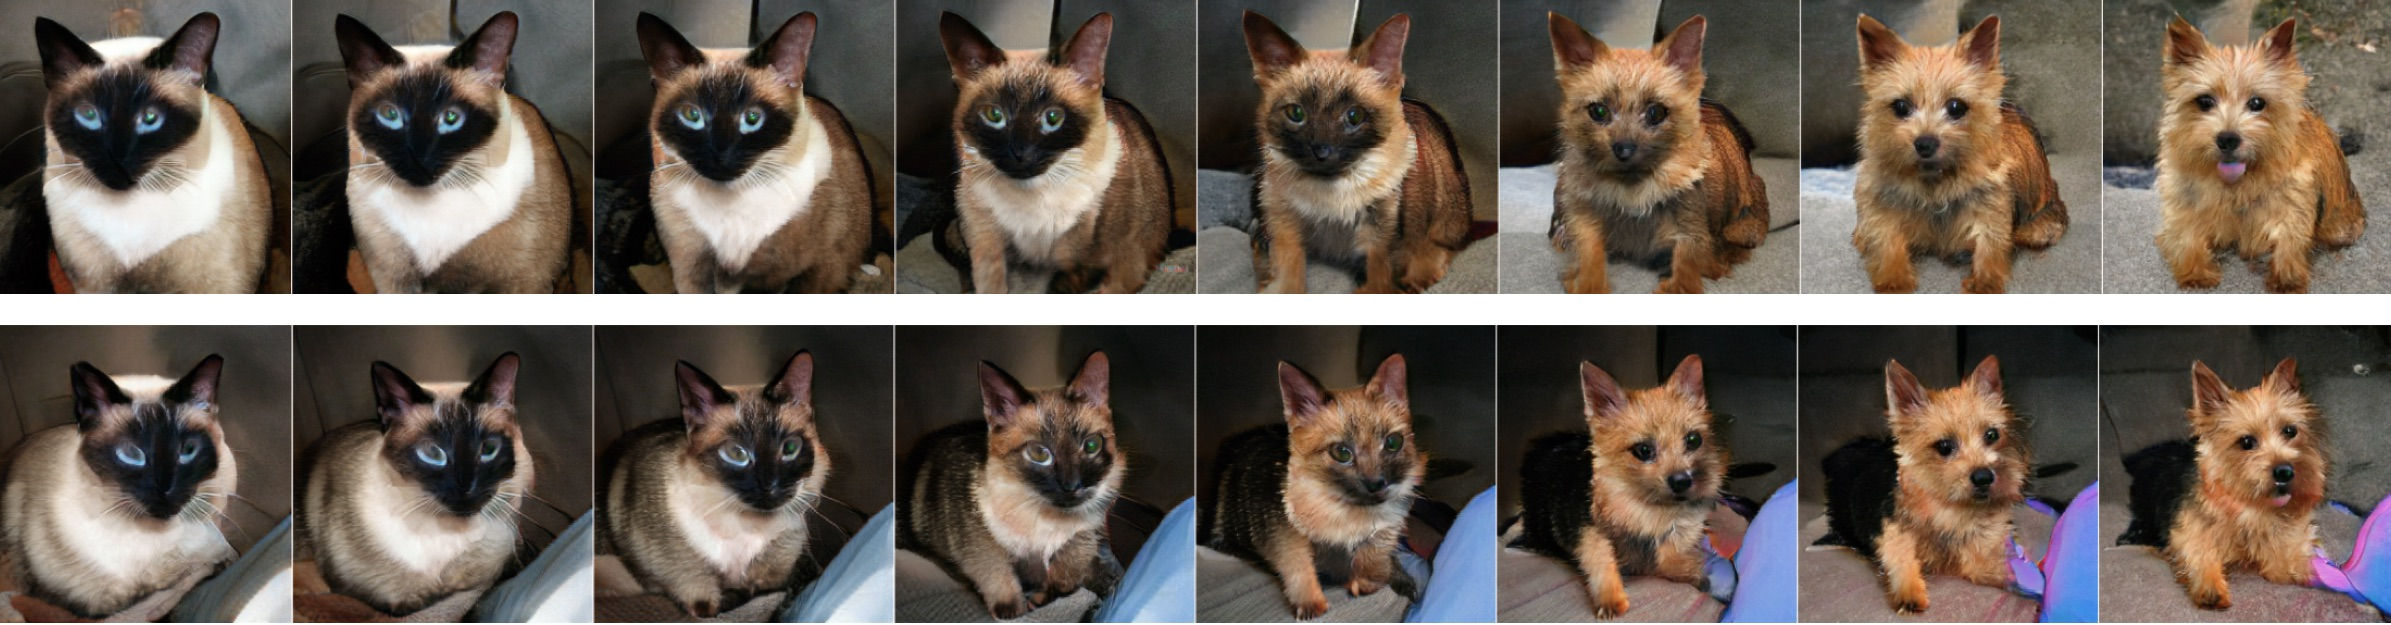
\includegraphics[width=.97\linewidth]{deepfake.jpg}
\caption{Deux suites d'images synthétiques interpolant entre chats et chiens, obtenues avec BigGAN~\cite{brock2018large}. BigGAN est conditionné par les classes : cette information fait partie du conditionnement. Ces exemples illustrent la génération et l'interpolation, sans affirmer qu'il s'agit de chemins de transport optimal.}\label{fig:deepfake}
\end{figure}

Interpoler les variables latentes ou de conditionnement peut produire des transitions visuelles régulières, comme à la figure~\ref{fig:deepfake}. Ces chemins ne sont pas nécessairement des géodésiques de transport et ne restent pas toujours typiques de la distribution d'apprentissage. La plausibilité visuelle, la diversité, la fidélité à la loi cible et les résultats sur des données réservées sont des aspects distincts de la qualité d'un modèle génératif.
